\documentclass[useAMS,usenatbib]{mn2e}

\voffset=-0.8in

% Packages:
\usepackage{graphicx}
\usepackage{amsmath}
\usepackage{xspace}
\usepackage{dsfont}

% Bold symbols
\renewcommand{\btheta}{\boldsymbol{\theta}}
\newcommand{\bx}{\boldsymbol{x}}

% \onecolumn
%%%%%%%%%%%%%%%%%%%%%%%%%%%%%%%%%%%%%%%%%%%%%%%%%%%%%%%%%%%%%%%%%%%%%%%%%%%%%%

\title[Hierarchical Reverberation Mapping]
{Hierarchical Reverberation Mapping}
    
\author[Brewer and Elliott]{%
  Brendon~J.~Brewer$^{1}$\thanks{bj.brewer@auckland.ac.nz},
  Tom M. Elliott$^{1}$
  \medskip\\
  $^1$Department of Statistics, The University of Auckland, Private Bag 92019, Auckland 1142, New Zealand}

%%%%%%%%%%%%%%%%%%%%%%%%%%%%%%%%%%%%%%%%%%%%%%%%%%%%%%%%%%%%%%%%%%%%%%%%%%%%%%

\begin{document}
             
\date{To be submitted to MNRAS Letters}
             
\maketitle

\label{firstpage}

%%%%%%%%%%%%%%%%%%%%%%%%%%%%%%%%%%%%%%%%%%%%%%%%%%%%%%%%%%%%%%%%%%%%%%%%%%%%%%

\begin{abstract}
Reverberation mapping (RM) is an important technique in studies of active
galactic nuclei (AGN). The key idea of RM is to measure the time lag $\tau$
between variations in the continuum emission from the accretion disc
and subsequent response of the broad line region (BLR). The measurement of
$\tau$ is typically used to estimate the physical size of the BLR and is
combined with other measurements to estimate the black hole mass $M_{\rm BH}$.
A major difficulty with RM campaigns is the large amount of data needed to
measure $\tau$. Recently, \citet{2012MNRAS.427.2701F} introduced a new approach
to RM where the BLR light curve is sparsely sampled, but this is counteracted
by observing a large sample of AGN, rather than a single system.
The results are combined to infer properties of the sample of
AGN. In this letter we implement this method using a hierarchical
Bayesian model and contrast this with the results from the previous stacked
cross-correlation technique. We find that our inferences are more precise and
allow for more straightforward interpretation than the cross-correlation
technique.
\end{abstract}
galaxies:active --- methods: data analysis
\begin{keywords}

\end{keywords}

%%%%%%%%%%%%%%%%%%%%%%%%%%%%%%%%%%%%%%%%%%%%%%%%%%%%%%%%%%%%%%%%%%%%%%%%%%%%%%

\section{Introduction}
Reverberation mapping (RM) is an important technique for the study
of active galactic nuclei (AGN). The technique is based on the temporal
fluctuations of the central continuum source, and the subsequent response
of the broad line region (BLR) emission. The time delay between the continuum
and the broad line fluctuations provides an estimate of the size of the BLR
\citep{peterson}.

RM is a observationally intensive, requiring observations over a period of
a few tens of days \citep{2013ApJ...769..128B}. As a result, many authors have
studied the data analysis techniques involved in RM, and substantial
advances have been made in recent years.
The methods introduced range from those that attempt to infer the
transfer function \citep[the distribution of lags in a single object,
e.g.][]{1995ApJ...440..166K, 2011ApJ...735...80Z},
the velocity-resolved transfer function
\citep{2010ApJ...720L..46B}, or the physical structure of the BLR itself
\citep{pancoast, arp151, pancoast2, 2013arXiv1310.3907L}.

There are many subtleties involved in reverberation mapping, that we will ignore
for the purposes of this letter. We note them here for completeness. Firstly,
the mean lag $\bar{\tau} = \int \tau\Psi(\tau)\, d\tau$, where $\Psi(\tau)$
is the normalised transfer function, is not equal to $c$ times the mean radius of the BLR
distribution, $\bar{r} = \int \sqrt{x^2+y^2+z^2}\rho(x, y, z)\, d^3 \mathbf{x}$.
Secondly, the mean lag $\bar{\tau}$ is not equivalent to the peak of the
cross-correlation function, except in the case of very narrow
transfer functions. Direct physical modelling of the BLR resolves these
issues \citep{pancoast, arp151}.

Recently, \citet{2012MNRAS.427.2701F, 2013MNRAS.434L..16F} introduced an
innovative approach to reverberation mapping where the results from multiple
AGN can be combined to yield inferences about the entire sample of AGN,
despite the fact that the constraints on any individual AGN are poor. Rather
than accurately measuring $\tau$ in a single object, it is possible to roughly
measure $\tau$ for a large number of objects, and to infer properties about
the distribution of $\tau$ values in the sample of objects (and hence in
a broader population, if the sample can be considered representative).

We implement this idea with a Bayesian hierarchical model
\citep{2012arXiv1208.3036L}.
These models are becoming increasingly common in astrophysics and have been
used in a variety of different fields
\citep[e.g.][]{loredo, kelly, extreme_deconvolution, 2012AJ....143...90S, 2013arXiv1310.5177B, 2013AJ....146....7B}.

\section{Model Assumptions}
If the continuum light curve of an AGN
is described by a function $y(t)$, then the line
light curve $l(t)$ is given by
\begin{eqnarray}
l(t) &=& A \int_\tau \Psi(\tau)\left[y(t - \tau) + C\right] \, d\tau
\end{eqnarray}
where $\Psi(\tau)$ is the transfer function (assumed to be normalised),
and $A$ and $C$ are response
coefficients. The idea of reverberation mapping is to use noisy measurements
of $y(t)$ and $l(t)$ to infer the transfer function $\Psi(\tau)$ or a summary
of it such as the mean lag $\bar{\tau} = \int \tau\Psi(\tau) \, d\tau$.
Throughout this letter we consider $y(t)$ and $l(t)$ in flux
units, as opposed to magnitudes.

\section{Combining Inferences About Multiple Objects}
Consider a sample of $N$ objects, each of which has parameters $\theta_i$.
If the $i$th object is analysed on its own, the inference about 
its parameters $\theta_i$ is described by a posterior distribution
\begin{eqnarray}
p(\theta_i | x_i) \propto \pi(\theta_i)p(x_i | \theta_i)\label{eq:individual}
\end{eqnarray}
where $\pi(\theta_i)$ is the prior distribution and $p(x_i | \theta_i)$ is the
likelihood function. If $N$ objects are analysed separately, inferences can
be made about the diversity of $\theta_i$ across the sample. However, these
inferences may be incorrect due to the implicit assumption that the prior for
all of the $\{\theta_i\}$ is independent.
A hierarchical model may be used to overcome this problem.
Section~\ref{sec:single_object} describes the assumptions used for analysing
data from a single AGN.

In a hierarchical model, the prior for the parameters $\{\theta_i\}$ is created
by introducing hyperparameters $\alpha$ such that the joint prior for $\alpha$
and the $\{\theta_i\}$ is:
\begin{eqnarray}
p(\alpha, \theta_i) &=& p(\alpha)\prod_{i=1}^N p(\theta_i | \alpha)
\end{eqnarray}
The posterior distribution for
$\btheta = \{\theta_1, ..., \theta_N\}$ and the hyperparameters $\alpha$
given the data 
$\bx = \{x_1, ..., x_N\}$
should actually be
\begin{eqnarray}
p(\alpha, \btheta | \bx) &\propto&
p(\alpha)p(\btheta|\alpha)p(\bx | \btheta, \alpha)\\
&=& p(\alpha)\prod_{i=1}^N f(\theta_i|\alpha)p(x_i | \theta_i)
\end{eqnarray}
The marginal posterior distribution for the hyperparameters $\alpha$ is
\begin{eqnarray}
p(\alpha | \bx) &=&
\int p(\alpha, \btheta|\bx) \, d\btheta\\
&\propto& p(\alpha)\int \prod_{i=1}^N f(\theta_i|\alpha)p(x_i | \theta_i) d^N\theta\\
&\propto& p(\alpha) \prod_{i=1}^N \int f(\theta_i|\alpha)p(x_i | \theta_i) d\theta_i\\
&\propto& p(\alpha) \prod_{i=1}^N \int \frac{f(\theta_i|\alpha)}{\pi(\theta)}p(x_i | \theta_i) \pi(\theta_i)d\theta_i\\
&\propto& p(\alpha) \prod_{i=1}^N \mathds{E}\left[\frac{f(\theta_i|\alpha)}{\pi(\theta)}\right]
\end{eqnarray}
where the expectation is taken with respect to the individual object posterior
of Equation~\ref{eq:individual}, and thus can be estimated using posterior
samples from the posterior distributions for the individual objects.
This result enables us to reconstruct the
posterior distribution for the hyperparameters even though the individual object
inferences were made without the hierarchical structure in the prior. This is
essentially an importance sampling approximation to the hierarchical model.

Rather than
analysing all objects together, which can be very computationally expensive,
we can use the posterior distributions from Equation~\ref{eq:individual}
to reconstruct the results that would be obtained if we did analyse all
objects together with a hierarchical prior on the $\theta_i$ parameters.

\section{The Single Object Model}\label{sec:single_object}
The posterior distribution for the mean lag $\bar{\tau}$ of a single object
$i$ may be obtained
by fitting the following model. We assume, for simplicity, that
the transfer function is uniform
between limits $a$ and $b$, where $b > a$:
\begin{eqnarray}
\Psi(\tau) &=& \left\{
\begin{array}{lr}
\frac{1}{b-a}, & \tau \in [a,b]\\
0, & \textnormal{otherwise}s
\end{array}\right.
\end{eqnarray}
and our goal is to measure the mean lag:
\begin{eqnarray}
\bar{\tau} &=& \int \tau \Psi(\tau) \, d\tau\\
&=& \frac{1}{2}(b-a)
\end{eqnarray}

Note that inferring $\bar{\tau}$ from the data requires that we
marginalise over an infinite number of nuisance parameters describing the
behaviour of $y(t)$ at unobserved times \citep{pancoast}.
The prior for the underlying time variation of the continuum emission is
a continuous autoregressive process of order 1, or a CAR(1) model. These models
have been studied extensively for AGN variability
\citep[e.g.][]{2009ApJ...698..895K, 2011ApJ...735...80Z, 2013ApJ...765..106Z}.
This marginalisation can be done
either analytically or inside MCMC. We used the latter approach for simplicity.
We discretised
time using ten time bins per day, and have a discrete continuum light curve
$\mathbf{y} = \{y_1, ..., y_n\}$, included in the model as a set of unknown
parameters. The prior for these parameters is:
\begin{eqnarray}
p(y_i | y_{i-1},  \mu, a, \beta) \sim \mathcal{N}
\left(\mu + a\left(y_{i-1} - \mu\right), \beta^2\right)
\end{eqnarray}
for $i \geq 2$. This is the discrete AR(1) model from time series theory.
$\mu$ describes the mean level of the continuum light curve, $\beta$ controls
the size of the short-term fluctuations, and $a$ controls the correlation
timescale.

For the likelihood (or sampling distribution, really the prior for the data
given the parameters) we made the conventional gaussian assumption:
\begin{eqnarray}
Y_i &\sim& \mathcal{N}\left(y(t_{y_i}), \sigma_{y_i}^2\right)\\
L_i &\sim& \mathcal{N}\left(l(t_{l_i}), \sigma_{l_i}^2\right)
\end{eqnarray}

To implement the MCMC for a single object,
we implemented our model in the STAN sampler \citep{nuts}
and Diffusive Nested Sampling \citep{dnest}. Due to the large number of
parameters and some very strong correlations in the posterior distribution,
we found that Diffusive Nested Sampling was more effective than STAN.
Note the single-object model is already an improvement over standard
cross-correlation techniques and is similar to the approach used by
\citep{2011ApJ...735...80Z}.

\section{Demonstration on Simulated Data}
To test our hierarchical model, and compare it to the stacked cross-correlation
function, we simulated data from 100 AGN. The data for each object was
continuum flux measurements, once per day, for 100 days. The continuum fluxes
for each object oscillate around a mean value of 50 in arbitrary units, and the
standard deviation of the measurement noise is 1 (i.e. 2\%). The line data is measured on
only two days, with times selected from a uniform distribution between $t=50$
and $t=100$ days (i.e. corresponding to the latter half of the continuum data).
The flux of the line data is scaled to half that of the line data, and the
measurement noise is 0.25, or 1\%, on the line data. See Figure~\ref{fig:data}
for three illustrative data sets from the sample.

\begin{figure}
\begin{center}
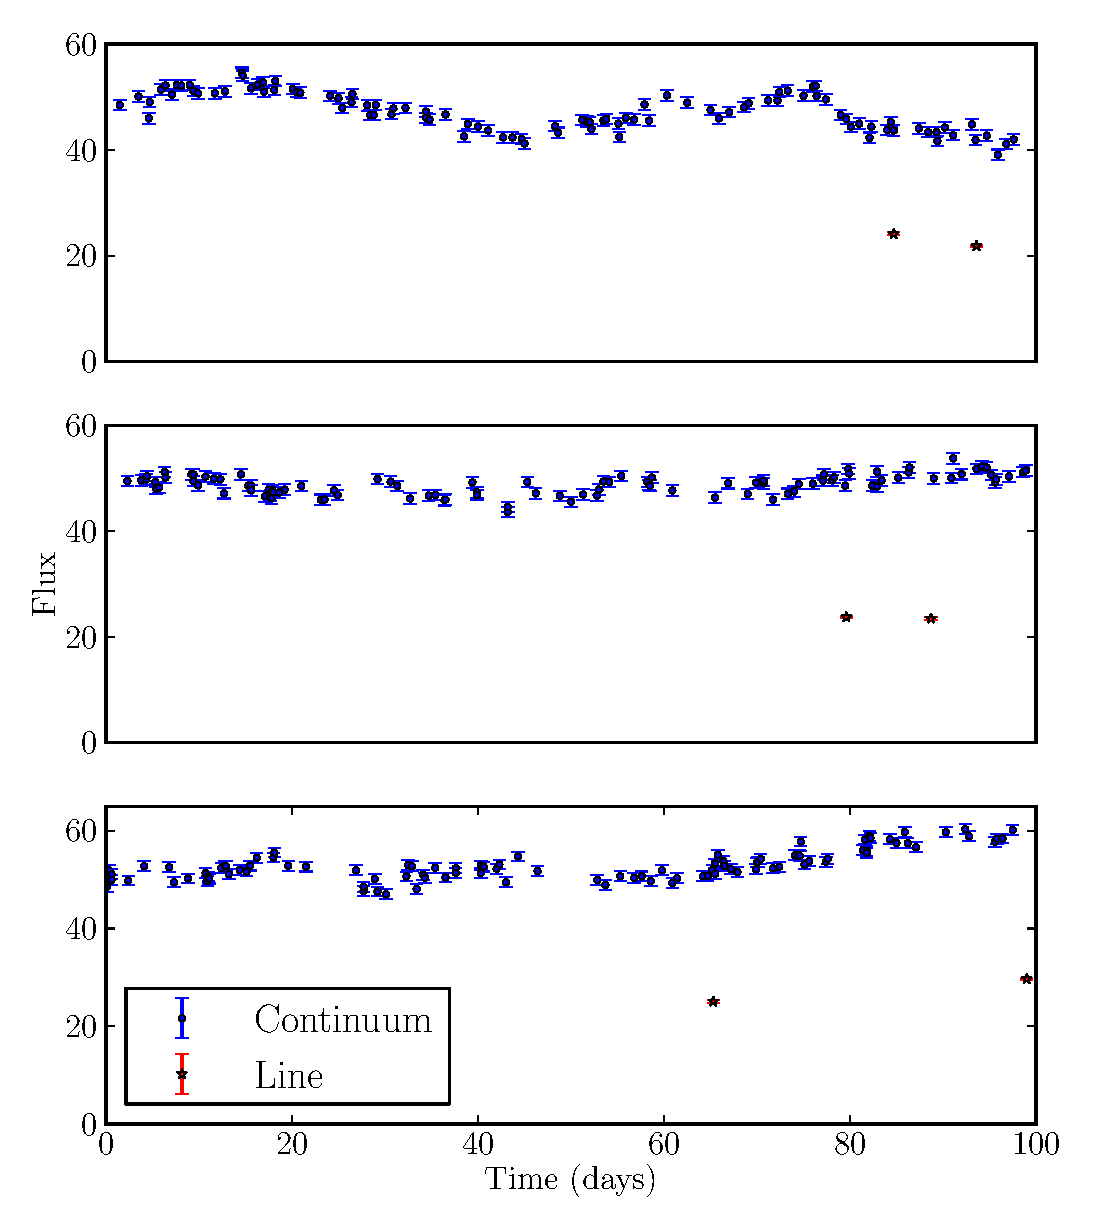
\includegraphics[scale=0.5]{Figures/data.eps}
\caption{Three simulated data sets, out of a total of 100.\label{fig:data}}
\end{center}
\end{figure}

The cross-correlation function for a single object is defined as follows. First,
the mean levels $\bar{y}$ and $\bar{l}$ of the continuum and line light curves,
are calculated (weighted by the reported size of the error bars on each
measurement):
\begin{eqnarray}
\bar{y} &=& \frac{\sum_{i=1}^{N_c} \left(y_i/\sigma_{y_i}^2\right)}{\sum_{i=1}^{N_c} \left(1/\sigma_{y_i}^2\right)}\\
\bar{l} &=& \frac{\sum_{i=1}^{N_l} \left(l_i/\sigma_{l_i}^2\right)}{\sum_{i=1}^{N_l} \left(1/\sigma_{l_i}^2\right)}
\end{eqnarray}

The cross correlation function, as a function of lags $\tau$, is then defined as:
\begin{eqnarray}
\textnormal{CCF}(\tau) =
\sum_{i=1}^{N_c} \sum_{j=1}^{N_l}
\left(\frac{(y_i - \bar{y})(l_j - \bar{l})}{\sigma_{y_i}^2\sigma_{l_j}^2}
\delta\left[\tau - (t_{l_j} - t_{y_i})\right]\right)
\end{eqnarray}
This can be understood as a set of delta-function spikes, one for each pair
of points (one point chosen from the continuum data, and one point from the
line data). The position of each spike depends on the time between the continuum
data point and the line data point, and the mass of each spike is proportional
to the continuum and line fluxes.

The stacked cross-correlation function for $N$ objects is sum of the CCFs
of the individual objects.
\begin{eqnarray}
\textnormal{SCCF}(\tau) &=&
\frac{1}{N} \sum_{i=1}^N
\left(
\frac{\textnormal{CCF}_i(\tau)}{\int \textnormal{CCF}_i(\tau) \, d\tau}
\right)
\end{eqnarray}
In Figure~\ref{fig:ccf},
we show the stacked CCF from the 100 simulated AGN data sets.

\begin{figure}
\begin{center}
\includegraphics[scale=0.5]{Figures/posterior.eps}
\caption{The joint posterior distribution for $\mu$ and $\sigma$, hyperparameters
describing the distribution of $\bar{\tau}$ values in the sample. The prior
distribution was uniform over the area shown.
The true solution is indicated by the white circle.\label{fig:posterior}}
\end{center}
\end{figure}

\begin{figure}
\begin{center}
\includegraphics[scale=0.35]{Figures/posterior2.eps}
\caption{The marginal posterior distribution for $\mu$, the 
hyperparameter describing the center of the distribution for
$\log_{10}\left(\bar{\tau}\right)$, is plotted as the solid line.
\label{fig:posterior2}}
\end{center}
\end{figure}

\begin{figure}
\begin{center}
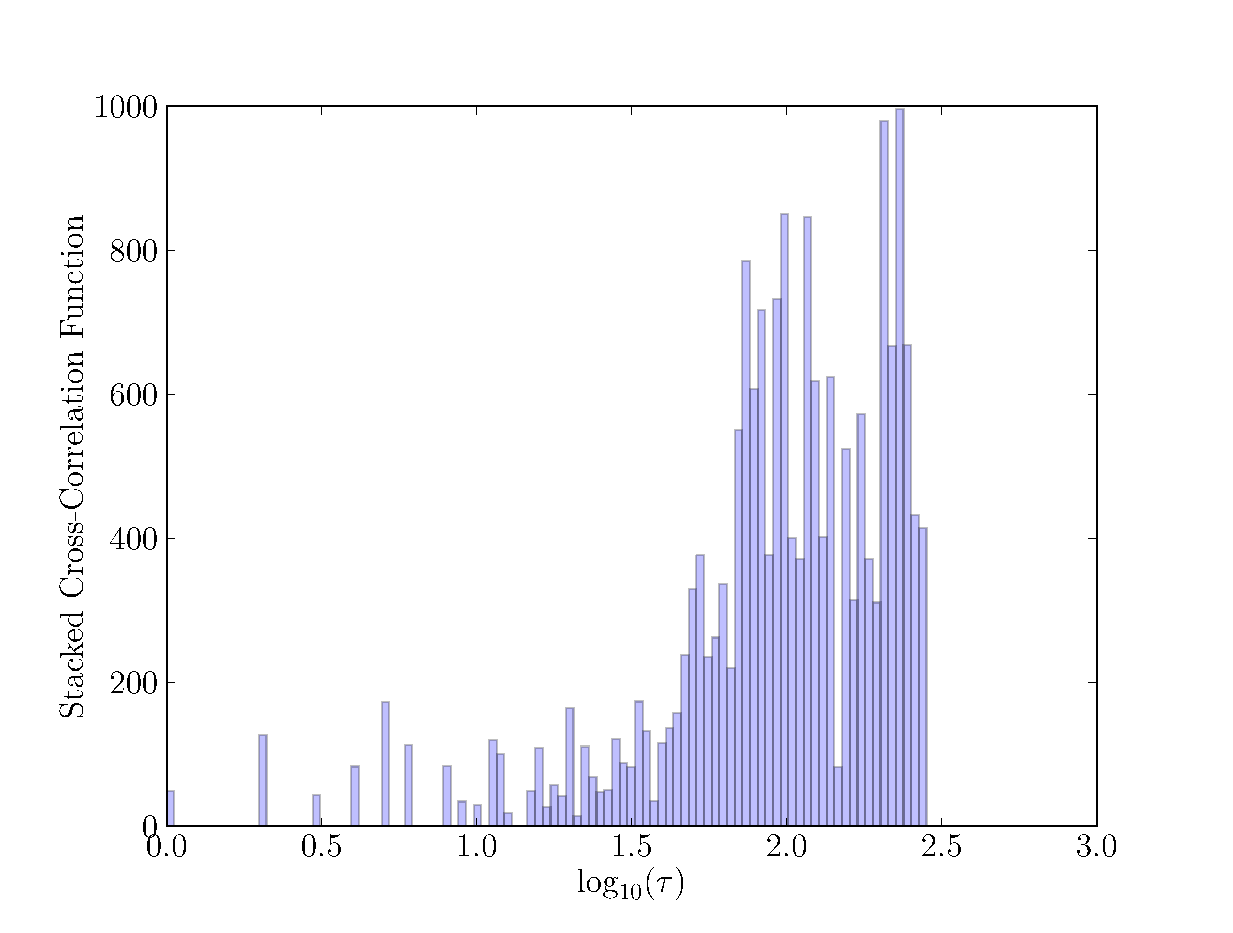
\includegraphics[scale=0.4]{Figures/ccf.eps}
\caption{The stacked cross-correlation function of the simulated data.
\label{fig:ccf}}
\end{center}
\end{figure}



\section*{Acknowledgements}
It is a pleasure to thank Tommaso Treu, Anna Pancoast (UCSB), and
Brandon Kelly (UCSB) for many
useful conversations about reverberation mapping. The STAN ({\tt mc-stan.org})
team provided helpful advice about the use of their software. BJB is partially
supported by the Marsden Fund (Royal Society of New Zealand).

\begin{thebibliography}{99}
\bibitem[\protect\citeauthoryear{Barth et al.}{2013}]{2013ApJ...769..128B} 
Barth A.~J., et al., 2013, ApJ, 769, 128 

\bibitem[\protect\citeauthoryear{Bentz et al.}{2010}]{2010ApJ...720L..46B} 
Bentz M.~C., et al., 2010, ApJ, 720, L46 

\bibitem[\protect\citeauthoryear{Brewer et al.}{2011}]{arp151} 
Brewer B.~J., et al., 2011, ApJ, 733, L33 

\bibitem[\protect\citeauthoryear{Brewer, P{\'a}rtay,
\& Cs{\'a}nyi}{2011}]{dnest} Brewer B.~J., P{\'a}rtay L.~B.,
Cs{\'a}nyi G., 2011, Statistics and Computing, 21, 4, 649-656. arXiv:0912.2380

\bibitem[\protect\citeauthoryear{Brewer, Foreman-Mackey, 
\& Hogg}{2013}]{2013AJ....146....7B} Brewer B.~J., Foreman-Mackey D., Hogg D.~W., 2013, AJ, 146, 7 

\bibitem[\protect\citeauthoryear{Brewer et al.}{2013}]{2013arXiv1310.5177B} 
Brewer B.~J., Marshall P.~J., Auger M.~W., Treu T., Dutton A.~A., 
Barnab{\`e} M., 2013, arXiv, arXiv:1310.5177 

\bibitem[\protect\citeauthoryear{Fine et al.}{2013}]{2013MNRAS.434L..16F} 
Fine S., et al., 2013, MNRAS, 434, L16 

\bibitem[\protect\citeauthoryear{Fine et al.}{2012}]{2012MNRAS.427.2701F} 
Fine S., et al., 2012, MNRAS, 427, 2701 

\bibitem[\protect\citeauthoryear{Hogg, Myers, 
\& Bovy}{2010}]{extreme_deconvolution} Hogg D.~W., Myers A.~D., Bovy J., 2010, ApJ, 725, 2166 

\bibitem[\protect\citeauthoryear{Kelly}{2007}]{kelly} Kelly 
B.~C., 2007, ApJ, 665, 1489 

\bibitem[\protect\citeauthoryear{Kelly, Bechtold, 
\& Siemiginowska}{2009}]{2009ApJ...698..895K} Kelly B.~C., Bechtold J.,
Siemiginowska A., 2009, ApJ, 698, 895 

\bibitem[\protect\citeauthoryear{Krolik 
\& Done}{1995}]{1995ApJ...440..166K} Krolik J.~H., Done C., 1995, ApJ, 440, 166 

\bibitem[\protect\citeauthoryear{Li et al.}{2013}]{2013arXiv1310.3907L} Li 
Y.-R., Wang J.-M., Ho L.~C., Du P., Bai J.-M., 2013, arXiv, arXiv:1310.3907 

\bibitem[\protect\citeauthoryear{Loredo}{2004}]{loredo} Loredo 
T.~J., 2004, AIP Conference Series, 735, 195 

\bibitem[\protect\citeauthoryear{Loredo}{2012}]{2012arXiv1208.3036L} Loredo 
T.~J., 2012, arXiv, arXiv:1208.3036 

\bibitem[\protect\citeauthoryear{Hoffman 
\& Gelman}{2011}]{nuts} Hoffman M.~D., Gelman A., 2011, arXiv, arXiv:1111.4246 

\bibitem[\protect\citeauthoryear{Pancoast, Brewer, 
\& Treu}{2011}]{pancoast} Pancoast A., Brewer B.~J., Treu T., 2011, ApJ, 730, 139 

\bibitem[\protect\citeauthoryear{Pancoast et 
al.}{2012}]{pancoast2} Pancoast A., et al., 2012, ApJ, 754, 49 

\bibitem[\protect\citeauthoryear{Peterson}{2008}]{peterson} 
Peterson B.~M., 2008, NewAR, 52, 240 

\bibitem[\protect\citeauthoryear{Shu et al.}{2012}]{2012AJ....143...90S} 
Shu Y., Bolton A.~S., Schlegel D.~J., Dawson K.~S., Wake D.~A., Brownstein 
J.~R., Brinkmann J., Weaver B.~A., 2012, AJ, 143, 90 

\bibitem[\protect\citeauthoryear{Zu et al.}{2013}]{2013ApJ...765..106Z} Zu 
Y., Kochanek C.~S., Koz{\l}owski S., Udalski A., 2013, ApJ, 765, 106 

\bibitem[\protect\citeauthoryear{Zu, Kochanek, 
\& Peterson}{2011}]{2011ApJ...735...80Z} Zu Y., Kochanek C.~S., Peterson B.~M., 2011, ApJ, 735, 80 



\end{thebibliography}



\end{document}

%%%%%%%%%%%%%%%%%%%%%%%%%%%%%%%%%%%%%%%%%%%%%%%%%%%%%%%%%%%%%%%%%%%%%%%%%%%%%%
